\documentclass{beamer}
\usepackage[utf8]{inputenc}

\usetheme{Madrid}
\usecolortheme{default}
\usepackage{amsmath,amssymb,amsfonts,amsthm}
\usepackage{txfonts}
\usepackage{tkz-euclide}
\usepackage{listings}
\usepackage{adjustbox}
\usepackage{array}
\usepackage{tabularx}
\usepackage{gvv}
\usepackage{lmodern}
\usepackage{circuitikz}
\usepackage{tikz}
\usepackage{graphicx}

\setbeamertemplate{page number in head/foot}[totalframenumber]

\usepackage{tcolorbox}
\tcbuselibrary{minted,breakable,xparse,skins}

\definecolor{bg}{gray}{0.95}
\DeclareTCBListing{mintedbox}{O{}m!O{}}{%
  breakable=true,
  listing engine=minted,
  listing only,
  minted language=#2,
  minted style=default,
  minted options={%
    linenos,
    gobble=0,
    breaklines=true,
    breakafter=,,
    fontsize=\small,
    numbersep=8pt,
    #1},
  boxsep=0pt,
  left skip=0pt,
  right skip=0pt,
  left=25pt,
  right=0pt,
  top=3pt,
  bottom=3pt,
  arc=5pt,
  leftrule=0pt,
  rightrule=0pt,
  bottomrule=2pt,
  toprule=2pt,
  colback=bg,
  colframe=orange!70,
  enhanced,
  overlay={%
    \begin{tcbclipinterior}
    \fill[orange!20!white] (frame.south west) rectangle ([xshift=20pt]frame.north west);
    \end{tcbclipinterior}},
  #3,
}
\lstset{
    language=C,
    basicstyle=\ttfamily\small,
    keywordstyle=\color{blue},
    stringstyle=\color{orange},
    commentstyle=\color{green!60!black},
    numbers=left,
    numberstyle=\tiny\color{gray},
    breaklines=true,
    showstringspaces=false,
}
%------------------------------------------------------------
%This block of code defines the information to appear in the
%Title page
\title %optional
{1.3.4}
%\subtitle{A short story}

\author % (optional)
{R Nikhil-AI25BTECH11025}

\begin{document}

\frame{\titlepage}
\begin{frame}{Question}
If $ A(1, 3), B(-1, 2), C(2, 5) $ and $ D(x, 4) $ are the vertices of a parallelogram \( ABCD \), then the value of $x$ is \underline{\hspace{2cm}}(10, 2012)
\end{frame}

\begin{frame}{Theoretical Solution}
In a parallelogram, the opposite sides are equal. Therefore, the length of side AC equals to the length of side BD:
\begin{align}
\vec{D} - \vec{B} = \vec{C} - \vec{A} \\
\vec{D} = \vec{B} + \vec{C} - \vec{A}
\end{align}

Substituting the coordinates:
\end{frame}

\begin{frame}{Theoretical Solution}
\begin{align}
\myvec{ x \\ 4 } = \myvec{ -1 \\ 2 } + \myvec{ 2 \\ 5 } - \myvec{ 1 \\ 3 } \\
                 = \myvec{ -1 + 2 - 1 \\ 2 + 5 - 3 } \\
                 = \myvec{ 0 \\ 4 }
\end{align}

This gives us the equations: 

\begin{align}
    x=0  \\
    4=4
\end{align}

\textbf{Answer:}  
\textbf{x=0}
\end{frame}

\begin{frame}[fragile]
\frametitle{Main C Code}
   \begin{lstlisting}
// main.c
#include <stdio.h>

// function declaration
int find_x(int Ax, int Ay, int Bx, int By, int Cx, int Cy, int Dy);

int main() {
    int Ax=1, Ay=3, Bx=-1, By=2, Cx=2, Cy=5, Dy=4;
    int x = find_x(Ax, Ay, Bx, By, Cx, Cy, Dy);

    printf("The value of x is: %d\n", x);

\end{lstlisting}
	\end{frame}

\begin{frame}[fragile]
\frametitle{Main C Code}
   \begin{lstlisting}
 // save coordinates to file for Python
    FILE *fp = fopen("coords.dat","w");
    fprintf(fp,"%d %d\n",Ax,Ay);
    fprintf(fp,"%d %d\n",Bx,By);
    fprintf(fp,"%d %d\n",x,Dy);
    fprintf(fp,"%d %d\n",Cx,Cy);
    fclose(fp);

    return 0;
}
\end{lstlisting}
	\end{frame}

\begin{frame}[fragile]
\frametitle{C Function}
   \begin{lstlisting}
// parallelogram.c
#include <stdio.h>

int find_x(int Ax, int Ay, int Bx, int By, int Cx, int Cy, int Dy){
int Dx=Bx+Cx-Ax;

    return Dx;
}
\end{lstlisting}
\end{frame}

\begin{frame}[fragile]
\frametitle{Python Code}
   \begin{lstlisting}
from ctypes import CDLL
import matplotlib.pyplot as plt

# load shared library
lib = CDLL("./libparallelogram.so")

# run C main program to generate coords.dat
import os
os.system("./main")
# read coords
coords = []
with open("coords.dat") as f:
    for line in f:
        x,y = map(int,line.split())
        coords.append((x,y))

# close polygon
coords.append(coords[0])

\end{lstlisting}
\end{frame}


\begin{frame}[fragile]
\frametitle{Python Code}
   \begin{lstlisting}
# plot
xs, ys = zip(*coords)
plt.plot(xs, ys, marker='o')
plt.text(1,3,"A(1,3)")
plt.text(-1,2,"B(-1,2)")
plt.text(0,4,"D(0,4)")
plt.text(2,5,"C(2,5)")
plt.title("Parallelogram ABCD")
plt.grid(True)
plt.savefig("/home/r-nikhil/ee1030-2025/ai25btech11025/matgeo/1.3.4/figs/plotc.png")
plt.show()

\end{lstlisting}
\end{frame}

\begin{frame}{Plot}
\begin{figure}[h!]
    \centering
    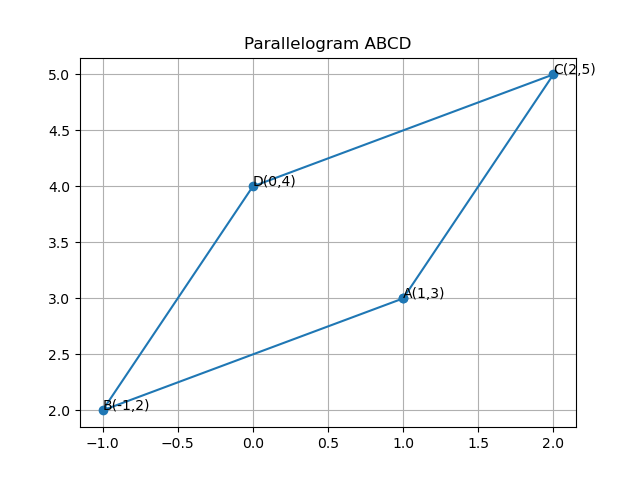
\includegraphics[height=0.6\textheight, keepaspectratio]{figs/plotc.png}
    \label{figure_1}
\end{figure}

\end{frame}
    
\end{document}
